\documentclass[11pt,a4paper]{article}
\usepackage[top=22mm,bottom=20mm,left=20mm,right=20mm,headheight=15pt]{geometry}
\usepackage[T1]{fontenc}
\usepackage{lmodern}
\usepackage{amsmath,amssymb,bm}
\usepackage{graphicx,booktabs,tabularx,array}
\usepackage{xcolor,enumitem,float,placeins,titlesec}
\titlespacing*{\section}{0pt}{10pt}{4pt}
\titlespacing*{\subsection}{0pt}{7pt}{3pt}
\usepackage{microtype,fancyhdr}
\usepackage[font=small,labelfont=bf]{caption}
\usepackage{listings}
\PassOptionsToPackage{hyphens}{url}
\usepackage[colorlinks=true,linkcolor=blue!45!black,urlcolor=blue!55!black,citecolor=blue!45!black]{hyperref}
\definecolor{navy}{HTML}{17354C}
\definecolor{teal}{HTML}{217A79}
\definecolor{pale}{HTML}{F2F5F7}
\hypersetup{pdftitle={Digital Watermarking for AI-Generated Media using DSP Techniques},
pdfauthor={Naman V Shetty, Ridhi Shakkar, Akarsh J, Mayur Soni}}
\pagestyle{fancy}
\fancyhf{}
\fancyhead[L]{\small EE313 | Digital Signal Processing}
\fancyhead[R]{\small IIT Indore}
\fancyfoot[C]{\thepage}
\setlength{\parindent}{0pt}
\setlength{\parskip}{3.5pt}
\setlength{\emergencystretch}{2em}
\setlength{\abovedisplayskip}{4pt plus 1pt minus 2pt}
\setlength{\belowdisplayskip}{4pt plus 1pt minus 2pt}
\setlength{\abovedisplayshortskip}{2pt}
\setlength{\belowdisplayshortskip}{2pt}
\setlist{itemsep=1pt,topsep=2pt}
\renewcommand{\arraystretch}{1.1}
\setlength{\textfloatsep}{8pt plus 2pt minus 2pt}
\setlength{\floatsep}{6pt plus 2pt minus 2pt}
\setlength{\intextsep}{6pt plus 2pt minus 2pt}
\captionsetup{skip=3pt}
\graphicspath{{figures/}}
\lstset{basicstyle=\ttfamily\scriptsize,breaklines=true,columns=fullflexible,
backgroundcolor=\color{pale},frame=single,rulecolor=\color{black!15},
showstringspaces=false,keepspaces=true}
\newcommand{\code}[1]{\texttt{\detokenize{#1}}}
\newcommand{\R}{\mathbb{R}}
\newcommand{\vect}[1]{\bm{#1}}
\begin{document}
\hypersetup{pageanchor=false}

\newgeometry{margin=12mm}
\begin{titlepage}
\centering
\vspace*{22mm}
{\fontsize{16}{20}\selectfont\bfseries INDIAN INSTITUTE OF TECHNOLOGY INDORE\par}
\vspace{7mm}
{\large EE313 --- Digital Signal Processing\par}
\vspace{22mm}
{\large Course Project Report\par}
\vspace{12mm}
{\color{navy}\fontsize{18}{22}\selectfont\bfseries Digital Watermarking for AI-Generated Media\par}
\vspace{5mm}
{\color{navy}\fontsize{15}{18}\selectfont\bfseries using DSP Techniques\par}
\vspace{22mm}
\rule{0.82\textwidth}{0.6pt}
\vspace{8mm}
\begin{tabular}{ll}
\textbf{Team member} & \textbf{Roll number} \\
\midrule
Akarsh J & 240002007 \\
Mayur Soni & 240002037 \\
Naman V Shetty & 240002043 \\
Ridhi Shakkar & 240002069 \\
\end{tabular}
\end{titlepage}
\restoregeometry

\pagenumbering{roman}
\hypersetup{pageanchor=true}
{\small\setlength{\parskip}{0pt}\tableofcontents}
\clearpage
\section*{Abstract}
\addcontentsline{toc}{section}{Abstract}
This project implements a keyed, invisible watermark for images and videos, with
AI-generated media provenance as its intended application. A short identifier is
embedded when media is published and recovered later using a secret key. The
system is a watermarking prototype, not a classifier of AI-generated content.

The image pipeline combines a three-level Haar discrete wavelet transform (DWT),
orthonormal block discrete cosine transforms (DCT), and spread-transform dither
modulation (STDM). Message bits are represented by parity quantization lattices
along keyed pseudo-noise projections. Convolutional coding and soft-decision
Viterbi decoding improve reliability, and CRC and HMAC checks determine whether
the recovered payload is valid. Video processing adds a temporal Haar
decomposition and combines soft scores from repeated observations across frames.

Experiments were regenerated from the project code on 15 November 2026. With the
default configuration, a $512\times512$ AI-generated forest-and-river image carrying an 18-byte
message achieved \textbf{46.97 dB PSNR}, \textbf{0.9973 SSIM}, and zero payload bit
error rate without an attack. Recovery also succeeded after JPEG compression,
additive noise, Gaussian blur, and registered scaling. Rotation, median filtering,
and cropping failed on this image. A second SpaceX rocket photograph achieved 47.47 dB PSNR
and 0.9904 SSIM; registered rotation passed there, while cropping failed. A separate
24-frame video test recovered its payload after H.264/H.265 recompression and the
implemented temporal attacks. A strength sweep demonstrates the central DSP
trade-off: increasing quantization spacing improves robustness at the cost of
greater signal distortion.

The evaluation uses one AI-generated nature image, one rocket photograph, and a
synthetic video rather than a representative dataset. Its conclusions therefore
establish a reproducible proof of concept, not general performance guarantees or
a complete provenance system.

\textbf{Keywords:} digital watermarking, multirate filter banks, Haar wavelets,
DCT, spread spectrum, quantization, error correction, video signal processing.
\clearpage
\pagenumbering{arabic}

\section{Introduction and project objectives}
AI-generated images and videos can be copied, recompressed, or distributed without
their original metadata. A watermark embeds an identifier within the media signal
itself: a trusted producer associates the identifier with an external record and
applies the watermark before release, and a verifier with the same key later
attempts recovery.

The project investigates three competing requirements:
\begin{enumerate}
\item \textbf{Imperceptibility:} the watermark should cause little visible distortion.
\item \textbf{Robustness:} the payload should survive selected processing operations.
\item \textbf{Capacity:} enough coefficients must remain available for useful data,
including framing and error-correction overhead.
\end{enumerate}
The implementation modifies transform coefficients rather than pixel
least-significant bits. It does not train a neural network, embed a visible logo,
or modify an AI generator. The payload is a short byte string, such as an asset
identifier. A missing watermark cannot establish that content is human generated,
and a valid watermark alone does not establish the truth of a scene.

\subsection{DSP concepts demonstrated}
\begin{table}[H]
\centering\footnotesize
\begin{tabularx}{\textwidth}{>{\raggedright\arraybackslash}p{0.30\textwidth}>{\raggedright\arraybackslash}X}
\toprule
Concept & Role in this project \\
\midrule
Discrete-time, multidimensional signals & Images are 2-D sampled signals; video adds a temporal axis. \\
Multirate filter banks & Haar low/high-pass filtering and downsampling create wavelet sub-bands. \\
Orthogonal transforms & DWT and DCT provide invertible coefficient representations for controlled modification. \\
Correlation and spread spectrum & PN projections distribute each bit across several coefficients. \\
Quantization & Two interleaved lattices encode binary decisions in coefficient space. \\
Noise and filtering & Compression, AWGN, blur, and resampling form practical distortion channels. \\
Temporal analysis and combining & Haar frame pairing and soft-score averaging exploit repeated evidence. \\
Signal fidelity measurement & MSE, PSNR, SSIM, and BER quantify quality and recovery. \\
\bottomrule
\end{tabularx}
\caption{Connection between the implementation and EE313 concepts. Error correction is a supporting digital-communications concept; CRC/HMAC provide integrity checks rather than signal transforms.}
\end{table}

\section{System architecture}
The embedding path has a signal branch and a message branch. The signal branch
provides transform-domain carriers. The message branch adds a header, error
protection, and authentication information. A secret key controls carrier order,
PN sequences, dither, and whitening. Figure~\ref{fig:pipeline} summarizes the image
path; the video path reuses this spatial processing inside temporal low-pass planes.
\begin{figure}[H]
\centering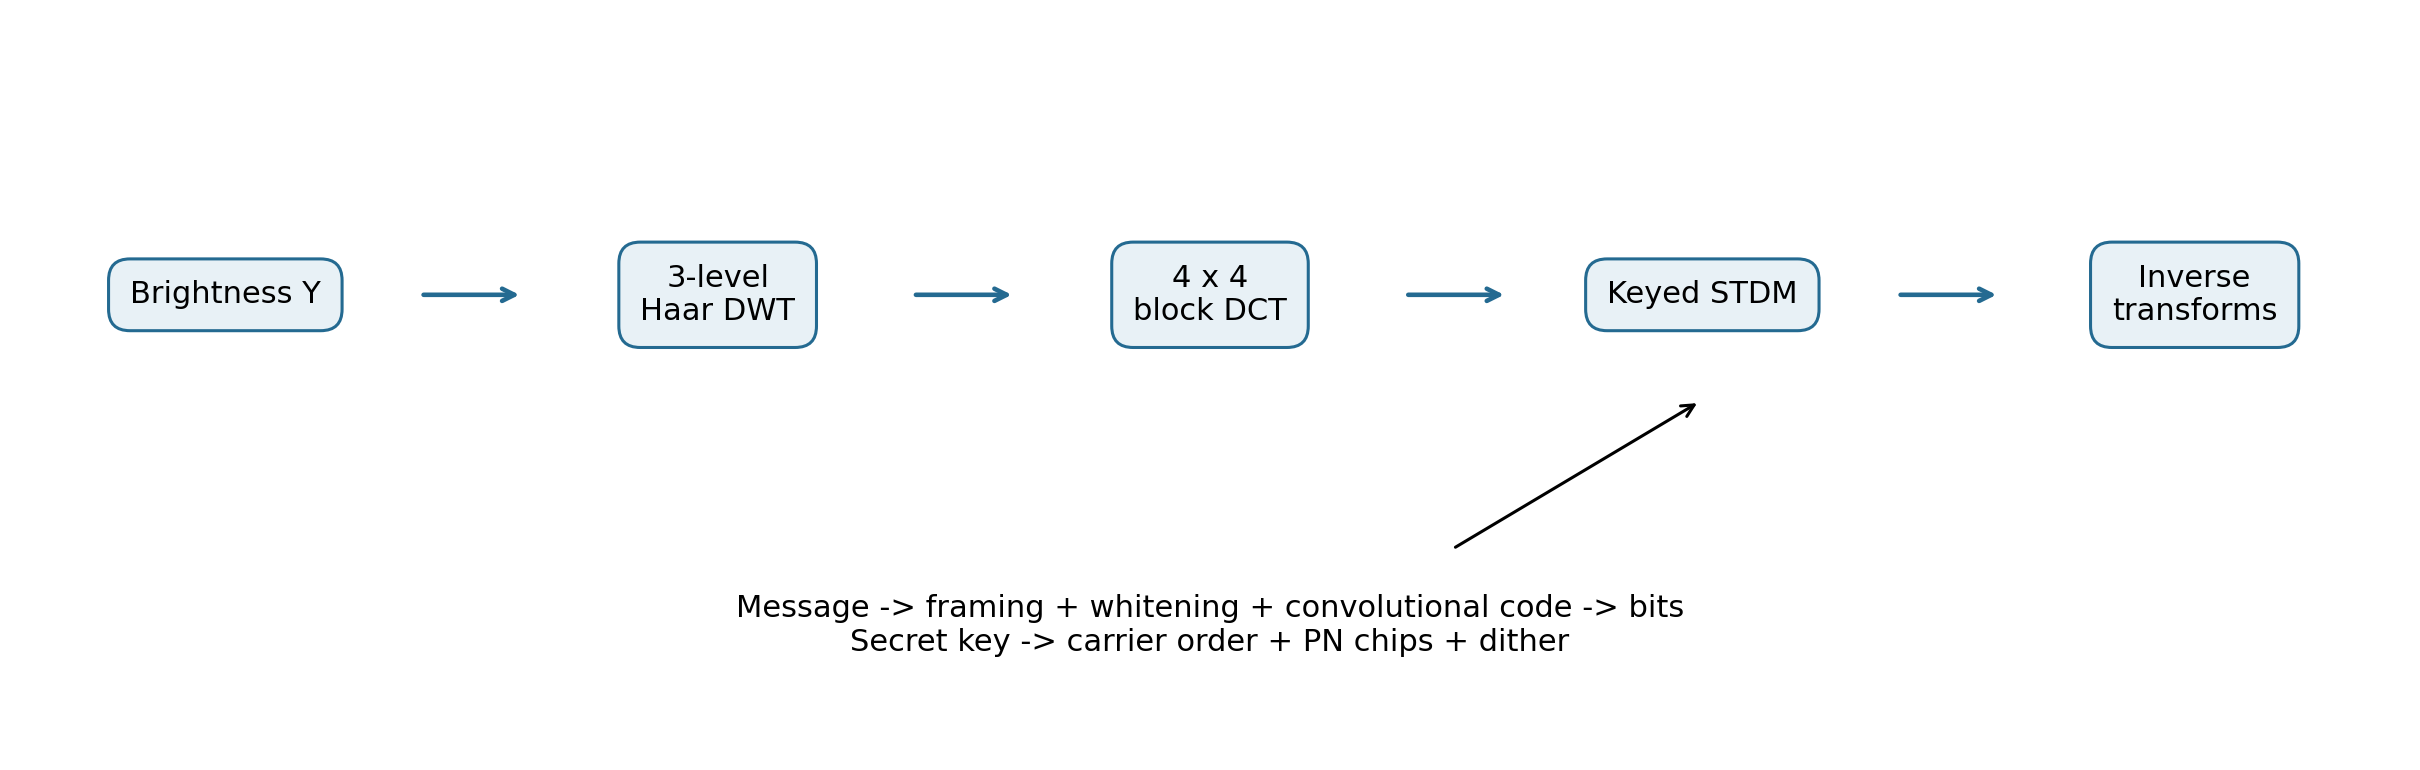
\includegraphics[width=.9\textwidth]{pipeline.png}
\caption{Image embedding architecture. The inverse transforms return the modified coefficients to the spatial domain. This figure is a schematic, not an experimental result.}
\label{fig:pipeline}
\end{figure}
Extraction applies the same analysis transforms, gathers keyed carriers, computes
soft bit scores, and decodes the payload. It needs the marked media, the key, and
matching configuration; a JSON sidecar can supply configuration, dimensions, and
expected payload length, but stores neither the key nor the plaintext message. The
geometric registration experiments additionally use the original image, making
those cases \emph{semi-blind}.

\section{Spatial DSP theory and embedding method}
\subsection{Luminance processing and boundary handling}
For color inputs, OpenCV converts BGR pixels to YCrCb. Only the brightness plane
$Y[m,n]$ is modified; chroma is carried through the reconstruction. A commonly used
luminance relation is $Y\approx0.299R+0.587G+0.114B$, with integer rounding in the
implementation. This reduces direct color disturbance, although conversion
rounding can still change reconstructed RGB values.

For DWT level $L$ and DCT block width $B$, dimensions are reflect-padded to a multiple
of $M=2^LB$. With $L=3$ and $B=4$, $M=32$. Reflection avoids the abrupt boundary
of zero padding. The default wavelet extension mode is periodization (padding and
wavelet extension are distinct operations). Transforms use 64-bit floating point;
final pixels are rounded and clipped to $[0,255]$.

\subsection{Haar DWT as a multirate filter bank}
The Haar analysis filters are
\begin{equation}
h[n]=\frac{1}{\sqrt{2}}[1,1],\qquad
g[n]=\frac{1}{\sqrt{2}}[1,-1].
\end{equation}
Filtering followed by decimation by two creates an approximation sequence and a
detail sequence. Equivalently, for one pair of samples,
\begin{equation}
a[k]=\frac{x[2k]+x[2k+1]}{\sqrt{2}},\qquad
d[k]=\frac{x[2k]-x[2k+1]}{\sqrt{2}}.
\end{equation}
The inverse follows by addition/subtraction and preserves energy:
$a[k]^2+d[k]^2=x[2k]^2+x[2k+1]^2$, so this is an orthonormal, critically sampled,
perfect-reconstruction filter bank before coefficient modification.

For a $2\times2$ patch $\left[\begin{smallmatrix}a&b\\c&d\end{smallmatrix}\right]$,
separable row/column processing gives the repository's Haar convention:
\begin{align}
LL&=(a+b+c+d)/2,& LH&=(a+b-c-d)/2,\\
HL&=(a-b+c-d)/2,& HH&=(a-b-c+d)/2.
\end{align}
The code maps PyWavelets' $(cH,cV,cD)$ to $(LH,HL,HH)$; naming conventions depend on
axis order, so the equations above state the convention explicitly~\cite{pywt}.
Only $LL$ is decomposed again at the next level. For a $512\times512$ input, the
three approximation sizes are $256\times256$, $128\times128$, and $64\times64$.

The watermark uses the level-3 $LH$ and $HL$ detail bands, which capture directional
variation at a coarser scale than first-level details. This is a practical
compromise: changing the approximation can produce conspicuous distortion, while
fine detail is easily removed by filtering. It does not guarantee invariance to
compression or geometric changes.

\begin{figure}[H]
\centering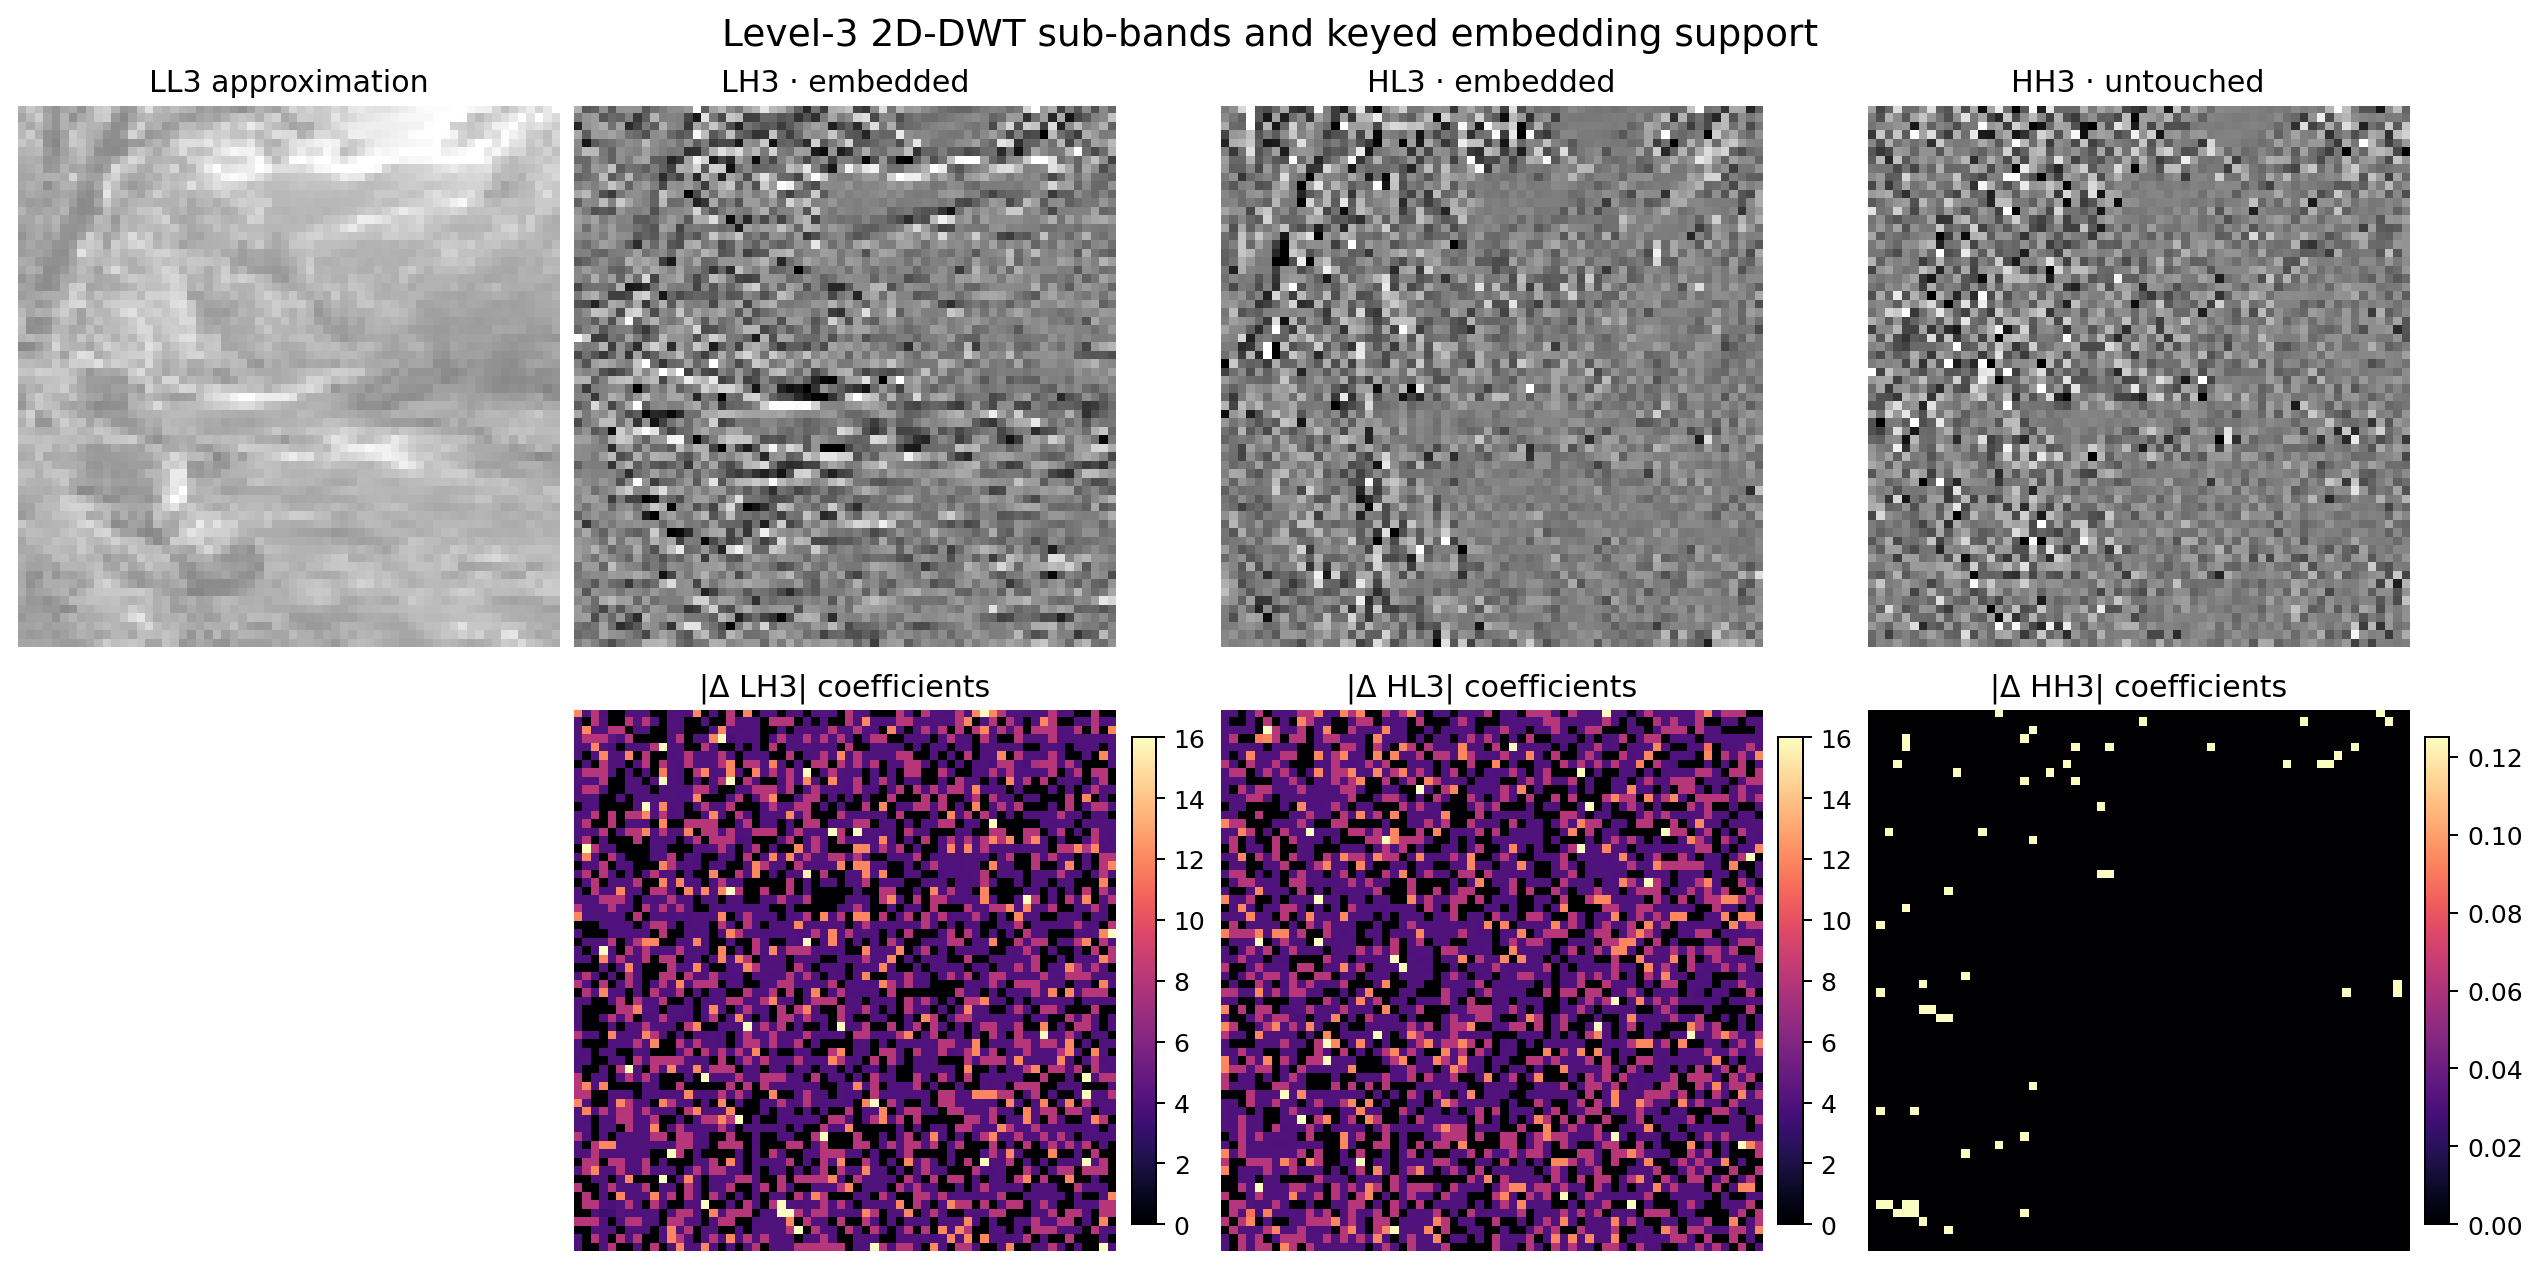
\includegraphics[width=.92\textwidth]{dwt_subbands.png}
\caption{Level-3 sub-bands of the measured test image and coefficient differences after reconstruction. The analysis directly modifies $LH_3$ and $HL_3$. Small changes seen when reanalyzing the nominally untouched $HH_3$ can arise from final pixel rounding and color conversion. Each difference panel uses its own scale.}
\label{fig:dwt}
\end{figure}

\subsection{Block DCT and frequency coefficient selection}
Each selected detail band is divided into $B\times B$ blocks. For a block $x[m,n]$,
the orthonormal two-dimensional DCT-II is
\begin{equation}
\begin{split}
C[u,v]={}&\alpha(u)\alpha(v)\sum_{m=0}^{B-1}\sum_{n=0}^{B-1}x[m,n]\\
&\cdot\cos\!\left(\frac{\pi(2m+1)u}{2B}\right)
\cos\!\left(\frac{\pi(2n+1)v}{2B}\right),
\end{split}
\end{equation}
where $\alpha(0)=\sqrt{1/B}$ and $\alpha(k)=\sqrt{2/B}$ for $k>0$.
The DC coefficient $C[0,0]$ describes the block average and is excluded. The default
$4\times4$ configuration uses \textbf{all 15 non-DC coefficients}, in zigzag order;
it does not select only a narrow mid-frequency subset of that DCT block.

The implementation calls SciPy's orthonormal DCT and inverse on the last two array
axes~\cite{scipy}. DWT localizes scale and orientation; block DCT adds a second
frequency representation within the selected bands. The transform itself does not
hide information: the controlled coefficient updates do.

For an orthonormal transform, Parseval's relation connects coefficient error energy
to signal error energy. Before clipping and rounding,
\begin{equation}
\|\delta x\|_2^2=\|\delta C\|_2^2.
\end{equation}
Thus coefficient changes have a measurable distortion cost, although final color
conversion, clipping, and rounding mean the reported RGB PSNR is not given by this
identity alone.

\subsection{Keyed PN projections and STDM}
Let $\vect{x}$ contain the selected DCT coefficients. A key-dependent permutation
groups them into disjoint chips $\vect{x}_i\in\R^{N_c}$. Each coded bit uses a balanced
pseudo-noise vector $\vect{p}_i\in\{-1,+1\}^{N_c}$, with half its entries positive and
half negative. The projection is
\begin{equation}
z_i=\frac{1}{N_c}\vect{p}_i^T\vect{x}_i,\qquad N_c=8.
\end{equation}
For bit $b\in\{0,1\}$, the dithered parity lattice is
\begin{equation}
\Lambda_b(d_i)=\left\{d_i+\Delta(2k+b):k\in\mathbb{Z}\right\},
\qquad 0\le d_i<\Delta.
\end{equation}
Adjacent points belonging to the same bit are $2\Delta$ apart. The two lattices
interleave with spacing $\Delta$. The nearest point of the required parity is chosen:
\begin{equation}
z_i'=\underset{q\in\Lambda_{b_i}(d_i)}{\arg\min}\,|z_i-q|,
\qquad
\vect{x}_i'=\vect{x}_i+(z_i'-z_i)\vect{p}_i.
\label{eq:embed}
\end{equation}
Since $\vect{p}_i^T\vect{p}_i=N_c$, substituting the update into the projection gives
exactly $z_i'$. The chip distortion is
\begin{equation}
\|\vect{x}_i'-\vect{x}_i\|_2^2=N_c(z_i'-z_i)^2.
\end{equation}
This connects quantizer spacing to distortion: increasing $\Delta$ separates
decision regions but generally requires larger changes. QIM and dither modulation
provide the underlying framework~\cite{chen}.

\textbf{Numerical illustration.} With $d_i=0$, $\Delta=12$, and $z_i=17$, bit 0
uses the nearest even-index lattice point, 24; bit 1 uses 12. The updates are
respectively $+7\vect{p}_i$ and $-5\vect{p}_i$. The actual implementation uses
key-dependent nonzero dithers and coefficient groups.

\subsection{Noise averaging and soft extraction}
If independent coefficient disturbances $\eta_j$ have zero mean and variance
$\sigma_c^2$, then the projection disturbance has variance
\begin{equation}
\mathrm{Var}\!\left(\frac{1}{N_c}\sum_{j=1}^{N_c}p_{ij}\eta_j\right)
=\frac{\sigma_c^2}{N_c}.
\end{equation}
This is an idealized model giving intuition for spreading; JPEG and interpolation
errors need not satisfy its independence assumptions. Larger chips also reduce
payload capacity.

Extraction computes $r_i=(\widehat{z}_i-d_i)/\Delta$ and distances to the nearest even
and odd integers, $e_i$ and $o_i$. The score is
\begin{equation}
s_i=\operatorname{clip}(|r_i-e_i|-|r_i-o_i|,-1,1).
\end{equation}
Negative scores favor bit 0 and positive scores favor bit 1; the magnitude is a
bounded confidence proxy, not a calibrated probability. Soft decisions preserve
information that a hard threshold would discard.

\subsection{Alternative SVD-QIM backend}
The project also offers $C=U\Sigma V^T$ decomposition of each selected DCT block.
It quantizes one chosen singular value using a keyed parity lattice and reconstructs
$C'=U\Sigma'V^T$. This is a separate backend, not a stage applied after STDM, and its carrier count
and capacity differ. The experiments in this report evaluate \textbf{STDM only}; they
do not establish an advantage over SVD-QIM.

\section{Payload coding and capacity}
\subsection{Framing, error correction, and validation}
The logical message consists of a 10-byte header and a body:
\begin{center}\small
\code{magic | version | flags | length | CRC32 | payload | HMAC tag}
\end{center}
Header fields occupy $2+1+1+2+4=10$ bytes. The default HMAC tag has eight bytes.
Header and body are independently whitened, then independently convolutionally
encoded. Whitening removes predictable bit patterns; it is not encryption. The default convolutional code has rate $1/2$, constraint length 7,
and octal generators $(171,133)$. Six zero tail bits terminate each block.

The Viterbi decoder searches a 64-state trellis using soft scores and traces back
from the zero state. Error correction attempts to recover bits; the CRC checks payload consistency and
the HMAC checks the key-dependent tag. A result is valid only when the header, CRC,
and HMAC checks all pass, so a low BER alone is not sufficient. The HMAC
authenticates payload bytes, not the host image.

\subsection{Worked default capacity calculation}
The two $64\times64$ bands each contain $16\times16=256$ DCT blocks. Therefore,
\begin{align}
N_{\mathrm{scalar}}&=2\cdot256\cdot15=7680,\\
N_{\mathrm{coded}}&=\left\lfloor\frac{7680}{8}\right\rfloor=960.
\end{align}
The 80-bit header consumes $2(80+6)=172$ coded carriers. The remaining 788 carriers
hold at most $\lfloor788/2\rfloor-6=388$ logical body bits, or 48 complete bytes.
Subtracting the 8-byte tag gives \textbf{40 payload bytes}.

The 18-byte experimental message plus its tag requires $26\cdot8=208$ body bits.
Its total encoded length is $172+2(208+6)=600$ bits, using $600\cdot8=4800$ scalar
coefficients; the remaining carriers are unused. Raw coefficient count is therefore
not the same as message capacity.

\section{Video: temporal DSP and synchronization}
\subsection{Temporal Haar analysis and synthesis}
For each pair of luminance frames, the temporal transform acts independently at
each spatial location:
\begin{equation}
L_t=\frac{Y_{2t}+Y_{2t+1}}{\sqrt{2}},\qquad
H_t=\frac{Y_{2t}-Y_{2t+1}}{\sqrt{2}}.
\end{equation}
$L_t$ captures common content and $H_t$ captures change between frames. The spatial
DWT--DCT--STDM pipeline embeds the same payload in each selected $L_t$. $H_t$ is
retained, and synthesis gives
\begin{equation}
\widehat{Y}_{2t}=\frac{\widehat{L}_t+H_t}{\sqrt{2}},\qquad
\widehat{Y}_{2t+1}=\frac{\widehat{L}_t-H_t}{\sqrt{2}}.
\end{equation}
A perturbation $\delta L_t$ contributes $\delta L_t/\sqrt{2}$ to both frames before
rounding; this shared perturbation motivates the design's reduced within-pair
flicker, which is not separately measured here. The video preset uses $\Delta=16$
(12 for images).

An eight-frame window supplies four low-pass planes; an incomplete last group is
padded by repeating its final frame, and only the original frame count is written.
Spatial and temporal processing form a separable spatio-temporal transform with no
motion model or motion-compensated wavelet stage.

\subsection{Voting, phase search, and encoding}
Repeated observations are combined before channel decoding:
\begin{equation}
\bar{s}_i=\frac{1}{T_s}\sum_{t=1}^{T_s}\operatorname{clip}(s_{i,t},-1,1).
\end{equation}
For independent, unbiased disturbances, averaging would reduce variance by
$T_s$; video observations are correlated, so this ideal gain is not assumed.
$T_s$ counts temporal low-pass score vectors, not independent trials.

After timing changes the extractor can search starting phases 0 through 7, ranking
candidates by validation and confidence; a valid phase-0 result returns early.
FFmpeg encodes H.264 or H.265 with keyframes aligned to the embedding-group
interval. Audio can be remuxed when present (the synthetic fixture has none).

\subsection{Geometric registration for images}
Rotation and resizing alter coefficient locations and hence keyed carrier
synchronization. The image extractor can align an attacked image to an original
reference using ORB matches and RANSAC similarity estimation, with homography and
ECC affine fallbacks. The registered image is then transformed and decoded.
Registration is an auxiliary computer-vision stage; DWT and DCT alone do not make
the watermark rotation- or crop-invariant, and interpolation cannot restore
information removed by cropping.

\section{Implementation and experimental methodology}
\subsection{Organization of the Python implementation}
\begin{table}[H]\centering\footnotesize
\begin{tabularx}{\textwidth}{>{\raggedright\arraybackslash}p{0.38\textwidth}>{\raggedright\arraybackslash}X}
\toprule
Module & Main responsibility \\
\midrule
\code{core/transforms.py} & Padding, DWT, block DCT, inverse transforms, SVD, temporal Haar. \\
\code{core/spread_spectrum.py} & Coefficient packing, zigzag order, keyed chips, STDM scores. \\
\code{core/qim.py} & Parity quantization and soft distances. \\
\code{core/payload.py} & Key expansion, framing, whitening, convolutional coding, Viterbi. \\
\code{core/embedder.py},\newline \code{core/extractor.py} & Image/video processing and recovery orchestration. \\
\code{core/media.py},\newline \code{core/video_io.py} & Image conversion, file I/O, FFmpeg encoding/remux. \\
\code{core/registration.py} & Reference-based geometric alignment. \\
\code{attacks/}, \code{benchmarks/} & Distortion channels, deterministic fixtures, result records. \\
\code{cli.py} & Embedding, extraction, capacity, and benchmark commands. \\
\bottomrule
\end{tabularx}
\caption{Mapping from report concepts to implementation. Configuration and metrics are in \code{core/config.py} and \code{core/metrics.py}.}
\end{table}

\subsection{Fixtures and parameters}
All measurements are from a new local run of source revision
\code{0b74cf3} on 15 November 2026. The primary image is an AI-generated forest-and-river
landscape created for this report and resized to $512\times512$ before embedding.
The second is a public-domain SpaceX rocket-launch photograph~\cite{rocket}, also
resized to $512\times512$. The payload is
\code{DSP-WATERMARK-2026} (18 UTF-8 bytes). The benchmark key is intentionally public.
The video fixture consists of 24 synthetic $512\times512$ frames at 12 fps with a
moving object and the 5-byte payload \code{VIDEO}.
Both images use the same configuration, payload, and attacks, so differences
between them reflect cover content and attack effects, not a changed setting.

\begin{table}[H]\centering\footnotesize
\begin{tabular}{lll}\toprule
Parameter & Image experiment & Video experiment \\\midrule
Spatial transform & Haar DWT, level 3 & Same \\
DCT block / bands & $4\times4$ / $LH_3,HL_3$ & Same \\
Carriers per block / chip & 15 / 8 & Same \\
Embedding step & $\Delta=12$ & $\Delta=16$ \\
ECC / HMAC tag & Rate $1/2$ / 8 bytes & Same \\
Temporal window & Not applicable & 8 frames \\
Baseline encoder & Lossless PNG / arrays & H.264, CRF 18, veryfast \\
Pixel format & BGR arrays & \code{yuv420p} output \\
\bottomrule\end{tabular}
\caption{Operating conditions. Video benchmarks override the general default encoder preset from medium to veryfast.}
\end{table}

\subsection{Quality and recovery metrics}
For $N$ scalar samples across all pixels and channels,
\begin{equation}
\mathrm{MSE}=\frac{1}{N}\sum_{j=1}^{N}(I_j-\widehat I_j)^2,
\qquad \mathrm{PSNR}=10\log_{10}\!\left(\frac{255^2}{\mathrm{MSE}}\right).
\end{equation}
Higher PSNR indicates less squared error. SSIM combines local luminance, contrast, and covariance:
\begin{equation}
\mathrm{SSIM}(x,y)=
\frac{(2\mu_x\mu_y+C_1)(2\sigma_{xy}+C_2)}
{(\mu_x^2+\mu_y^2+C_1)(\sigma_x^2+\sigma_y^2+C_2)}.
\end{equation}
The implementation uses an $11\times11$ Gaussian window with $\sigma=1.5$,
$C_1=(0.01\cdot255)^2$, and $C_2=(0.03\cdot255)^2$, then averages over channels.
The border is cropped by five pixels when dimensions permit.

\begin{equation}
\mathrm{BER}=\frac{\text{mismatched bits + missing/extra bits}}
{\max(\text{expected bit count},\text{extracted bit count})}.
\end{equation}
BER is evaluated on decoded payload bytes, not raw coefficient decisions. After a
failed decode the returned length may differ from the expected length, so a BER of
1 may indicate missing or misframed data rather than inversion of every bit.
Authentication validity is reported separately.

No-attack PSNR/SSIM measure watermark distortion; attacked rows also include the
attack's own distortion (geometric attacks are measured after registration) and are
not pure embedding-quality scores. Normalized correlation is implemented but not a
primary metric here, and no video PSNR, runtime, or flicker measurements are claimed.

\section{Measured image results}
\subsection{Visual quality and reconstruction error}
\begin{figure}[H]
\centering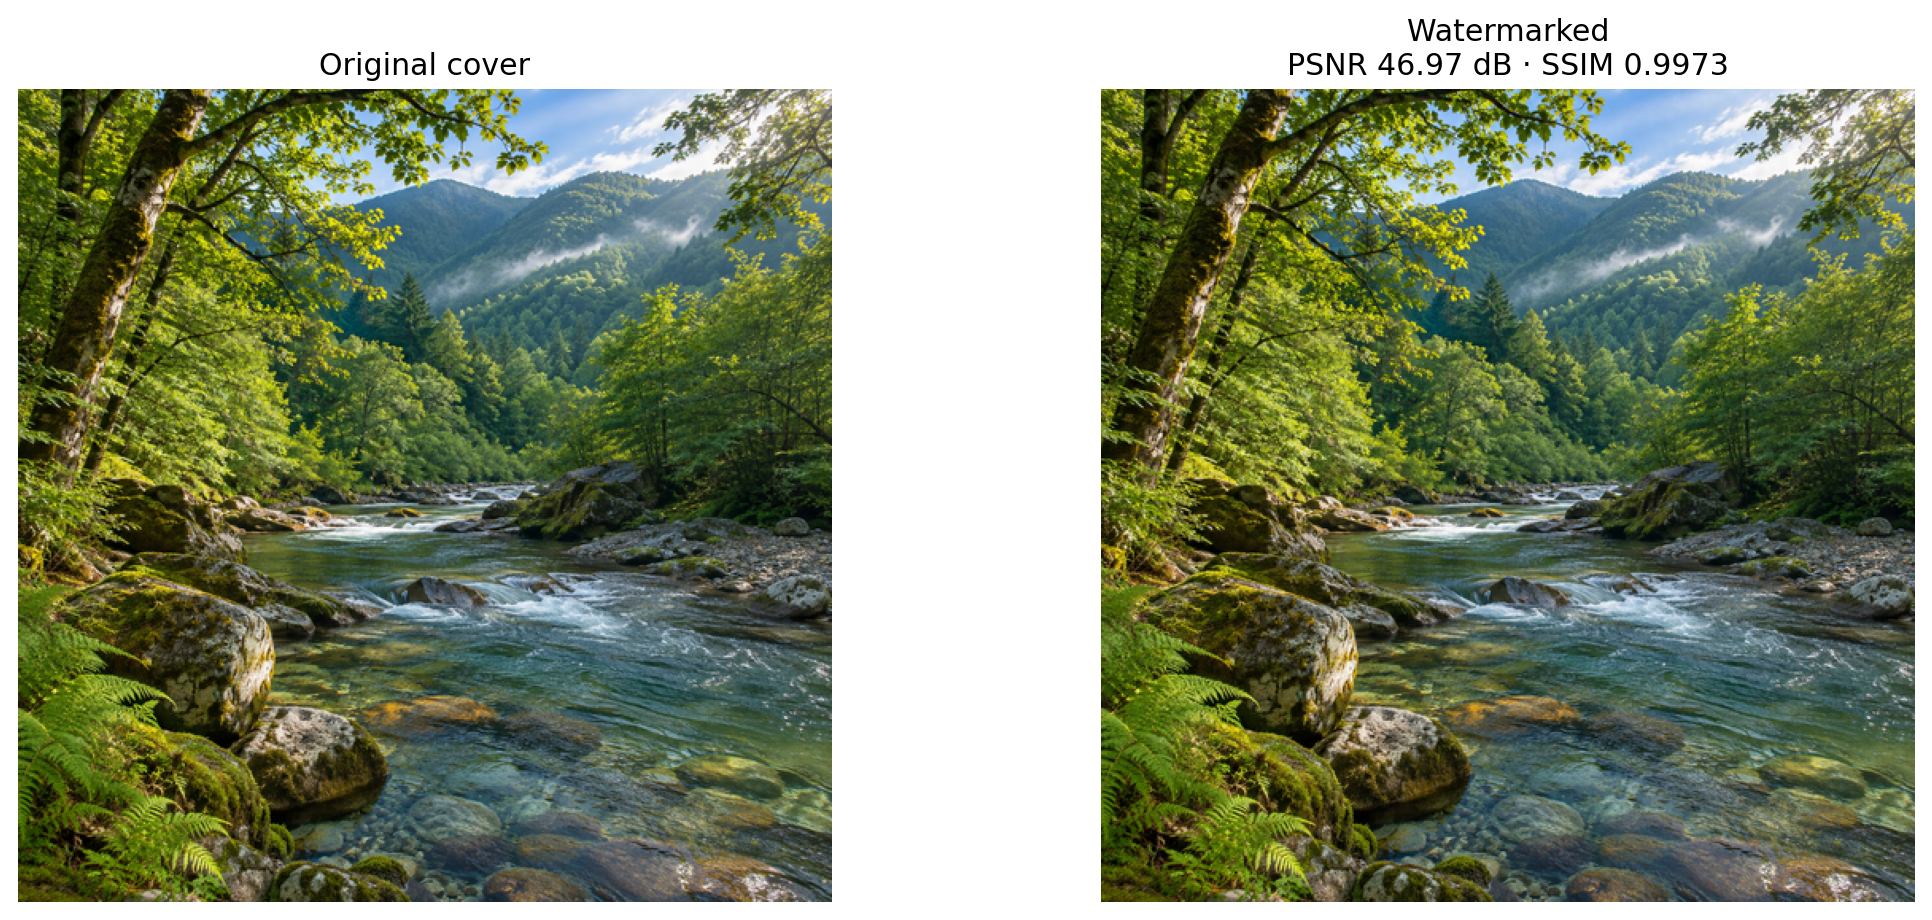
\includegraphics[width=.86\textwidth]{original_vs_watermarked.png}
\caption{Measured original and marked AI-generated nature image for the default 18-byte payload. PSNR is 46.97 dB and SSIM is 0.9973.}
\label{fig:comparison}
\end{figure}
\begin{figure}[H]
\centering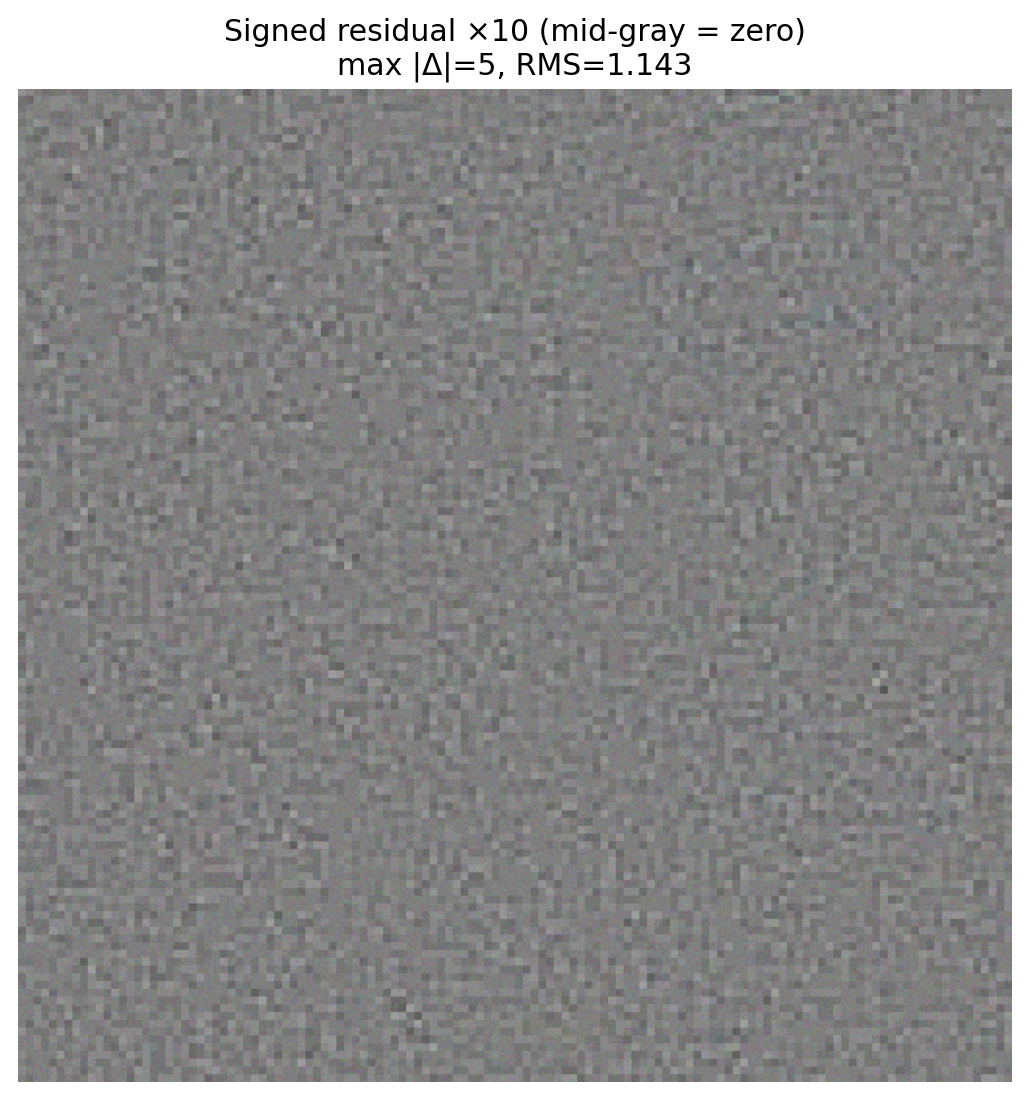
\includegraphics[width=.36\textwidth]{residual_x10.png}
\caption{Signed pixel residual multiplied by 10 and centered at gray. It is deliberately enhanced to reveal changes and does not represent the visible marked image. The residual reflects transform updates and final pixel/color quantization.}
\label{fig:residual}
\end{figure}
The clean payload was recovered exactly and all validation checks passed. High
PSNR and SSIM support low distortion for this fixture; they do not replace a human
perceptual study. Flat or different-content images may behave differently.

\subsection{Attack results and failure analysis}
\begin{table}[H]\centering\footnotesize
\begin{tabular}{lrrrr}
\toprule
Attack & PSNR (dB) & SSIM & BER & Valid \\
\midrule
No attack & 46.97 & 0.9973 & 0.0000 & Yes \\
JPEG Q=50 & 25.05 & 0.8024 & 0.0000 & Yes \\
Rotation $5^\circ$ (registered) & 24.40 & 0.8610 & 0.5486 & No \\
Median $3\times3$ & 24.35 & 0.7702 & 0.5694 & No \\
AWGN $\sigma=10$ & 28.21 & 0.8388 & 0.0000 & Yes \\
Gaussian blur $3\times3$ & 26.20 & 0.8530 & 0.0000 & Yes \\
Scale $0.75\times$ (registered) & 27.54 & 0.8956 & 0.0000 & Yes \\
Crop 90\% per axis (registered) & 20.28 & 0.8222 & 0.5139 & No \\
\bottomrule
\end{tabular}

\caption{Image attack benchmark. Registered rows use the original cover for alignment. Median and Gaussian kernels are $3\times3$; Gaussian blur uses $\sigma=0.8$. AWGN uses seed 7.}
\label{tab:attacks}
\end{table}
\begin{figure}[H]
\centering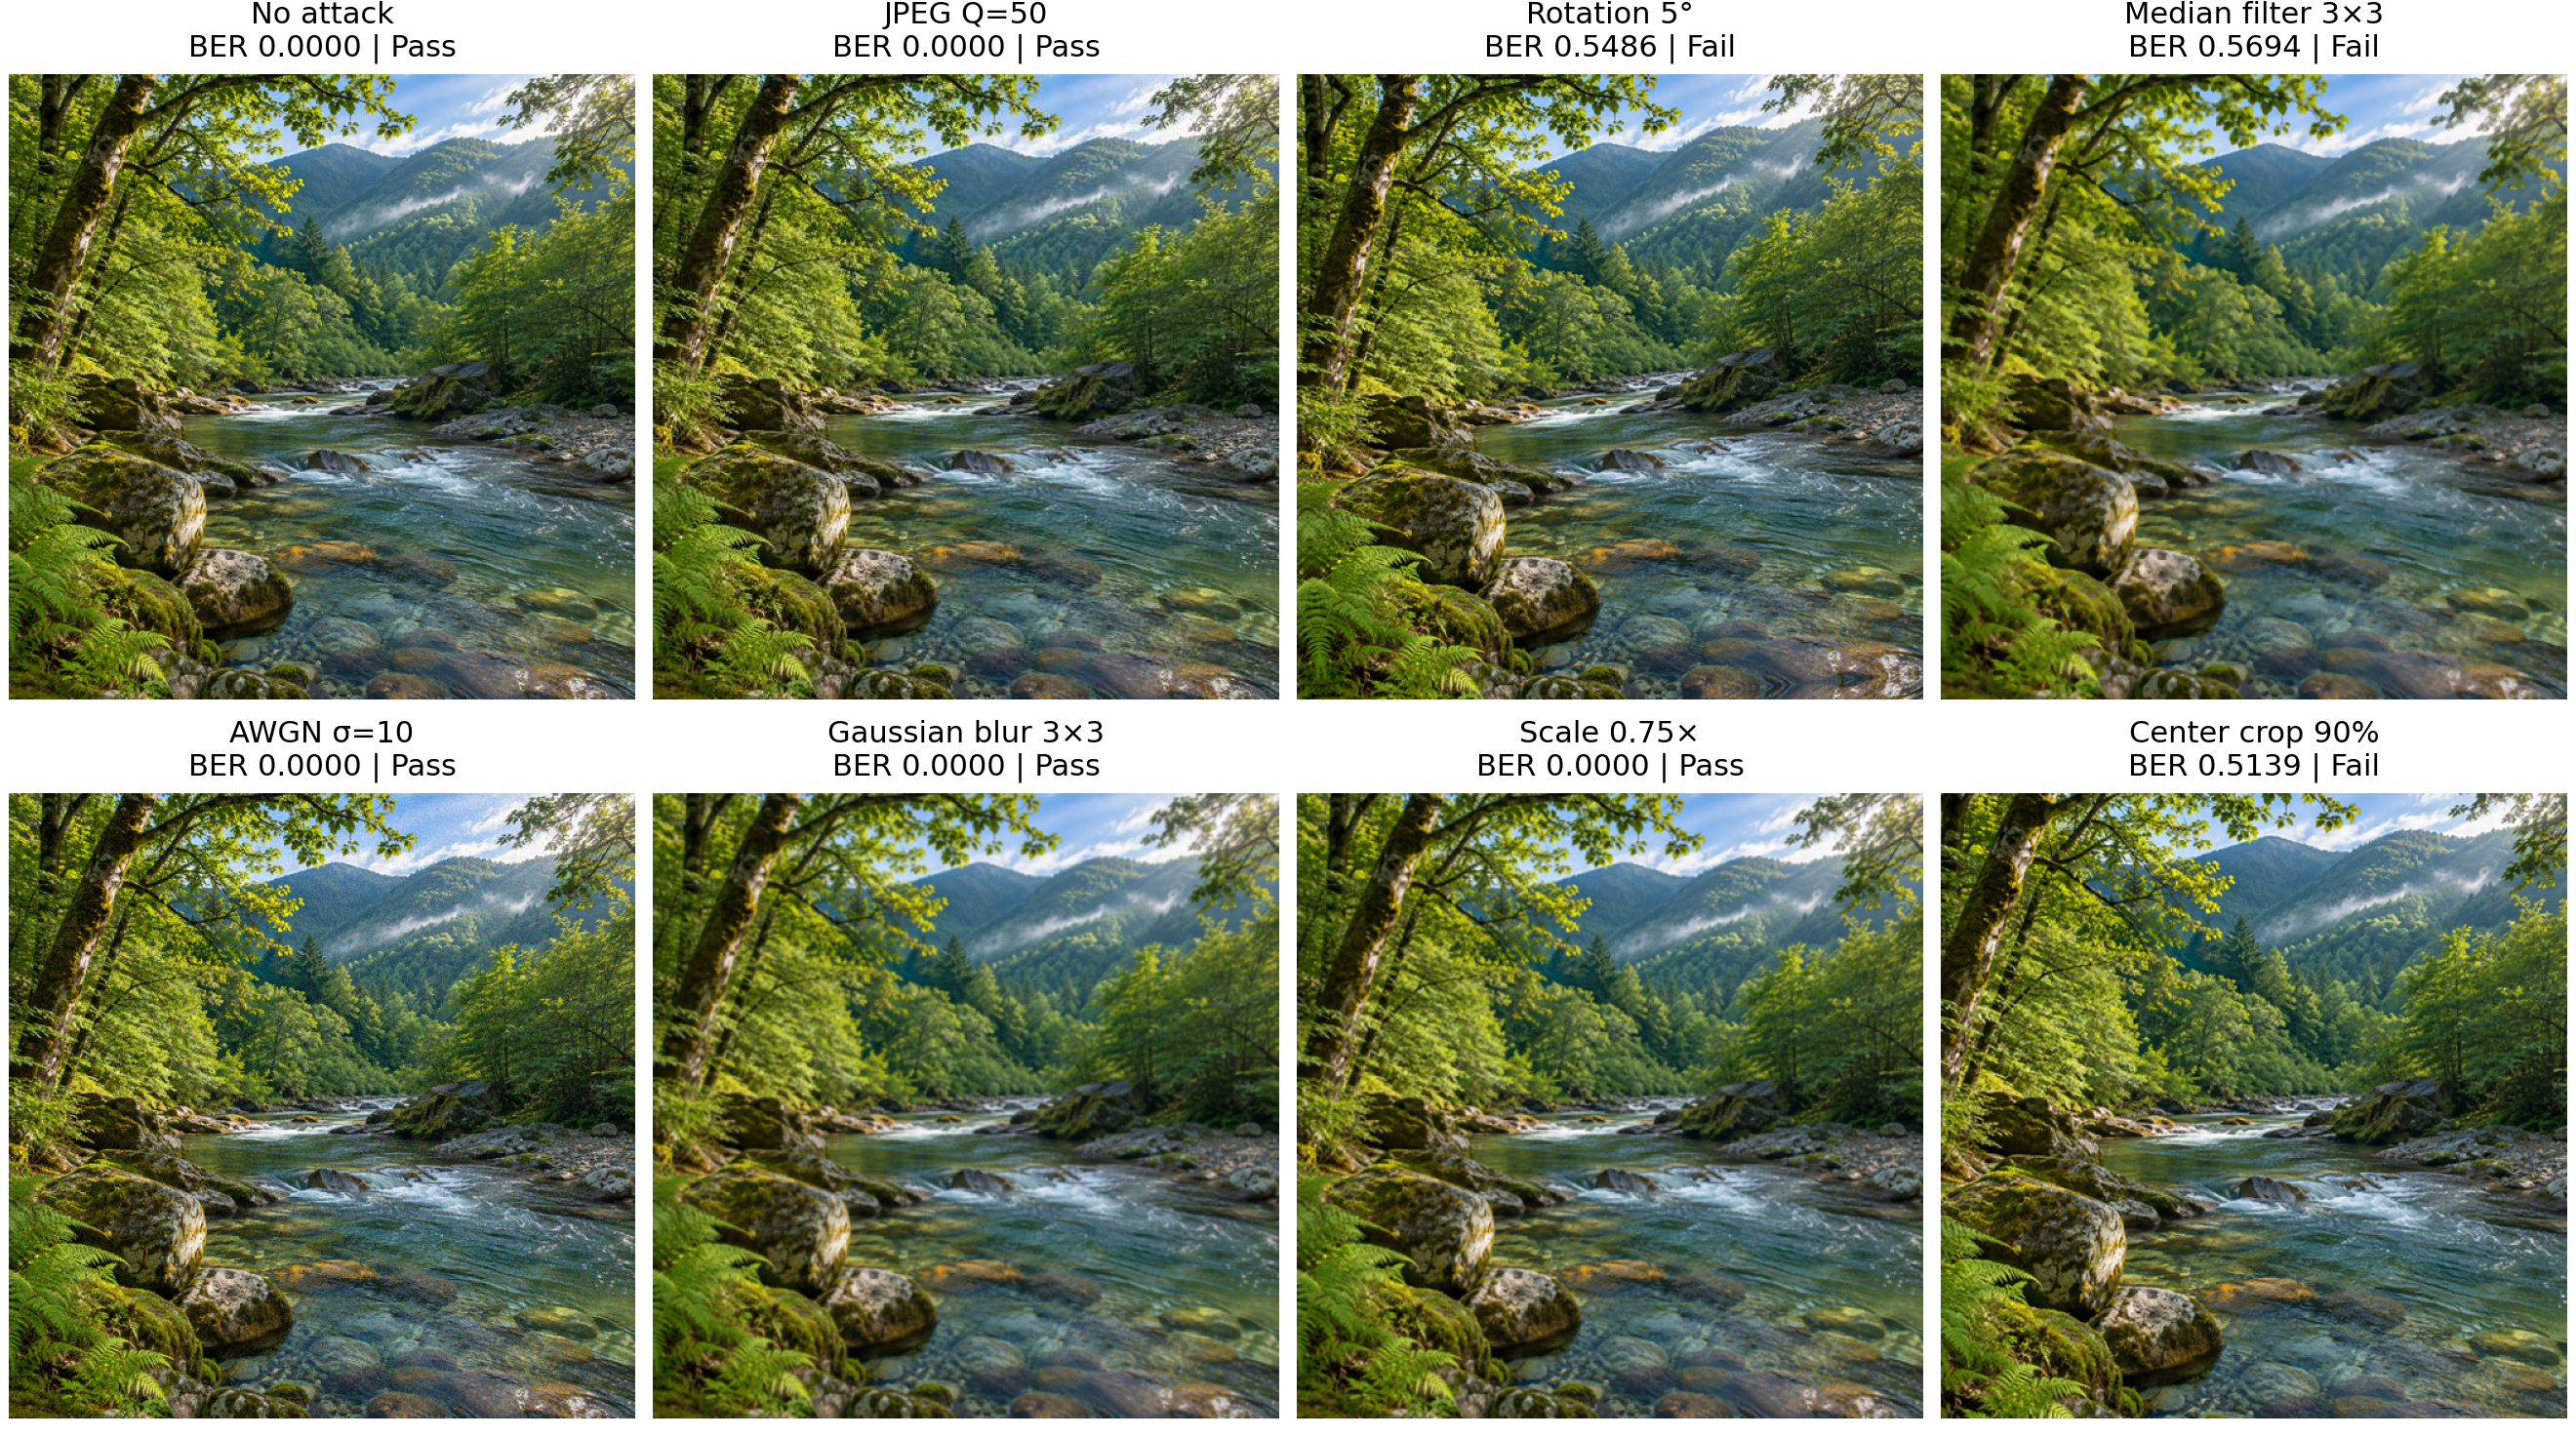
\includegraphics[width=.92\textwidth]{attack_montage.png}
\caption{Actual attacked images before optional reference alignment. Labels give the corresponding extraction results. BER for geometric attacks is measured after alignment, even though the panels show the input to alignment.}
\label{fig:attacks}
\end{figure}
JPEG, Gaussian blur, and additive noise disturb coefficients without destroying the
decoded payload in this run; spreading and soft decoding provide recovery margin.
Median filtering fails on the nature image, showing that nonlinear filtering can
alter selected coefficients more severely. Scale recovery depends on registration,
while rotation fails despite it. The crop retains 90\% of \emph{each} dimension
(about 81\% of the area), then resizes, and also fails with registration: removed
content and resampling disturb carrier correspondence. Reporting these failures
delimits the operating range of the implementation.

\subsection{Second image: SpaceX rocket photograph}
To test a different photographic cover, the same configuration, payload, key, and
attack suite were applied to a public-domain SpaceX rocket-launch photograph
supplied by scikit-image~\cite{rocket}, resized to $512\times512$ and saved as
\code{figures/rocket_original.png} to fix the input bytes.
\begin{figure}[H]
\centering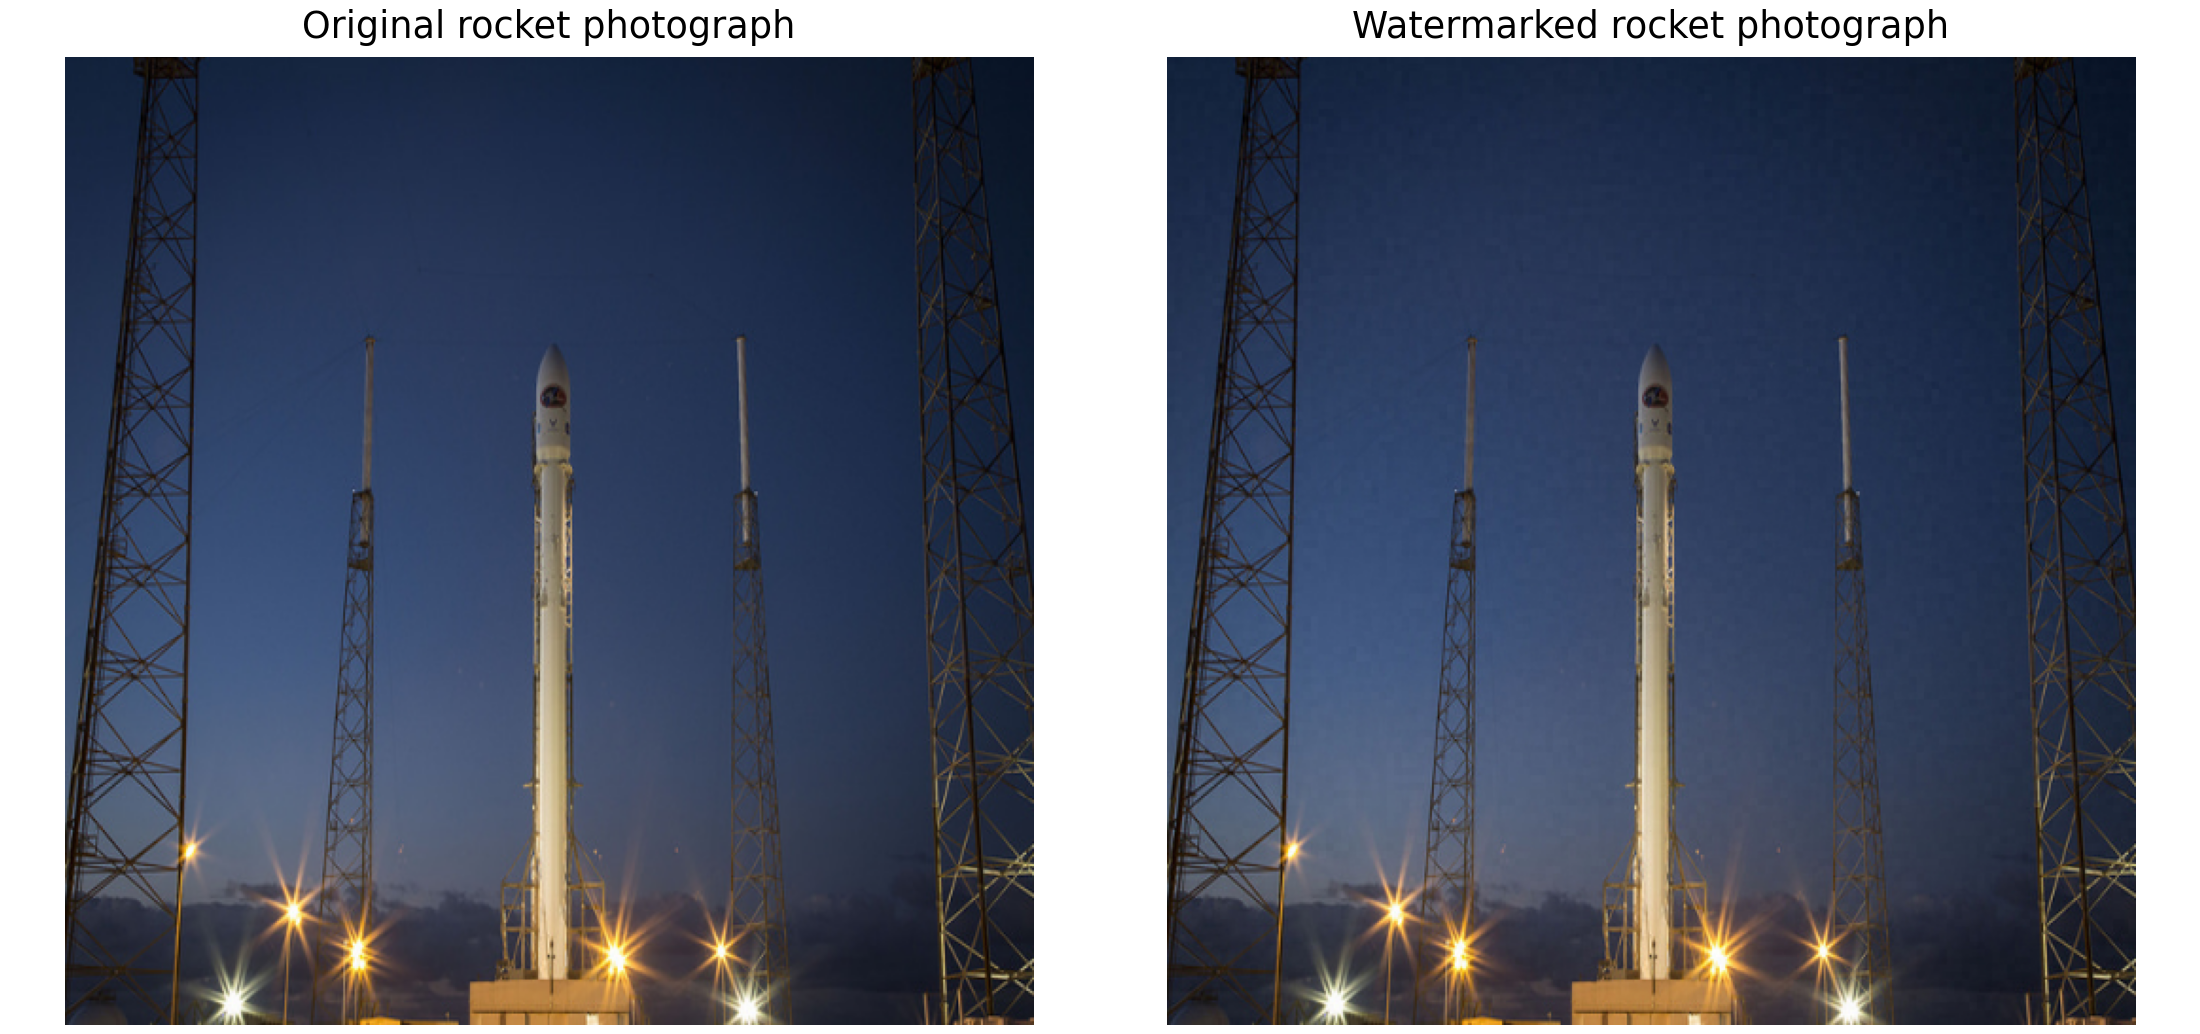
\includegraphics[width=.7\textwidth]{rocket_comparison.png}
\caption{Rocket photograph before and after watermark embedding. Clean PSNR is 47.47 dB, SSIM is 0.9904, BER is zero, and authentication passes.}
\label{fig:rocket}
\end{figure}
\begin{table}[H]\centering\footnotesize
\begin{tabular}{lrrrr}
\toprule
Attack & PSNR (dB) & SSIM & BER & Valid \\
\midrule
No attack & 47.47 & 0.9904 & 0.0000 & Yes \\
JPEG Q=50 & 32.15 & 0.8958 & 0.0000 & Yes \\
Rotation $5^\circ$ (registered) & 34.12 & 0.9706 & 0.0000 & Yes \\
Median $3\times3$ & 32.98 & 0.9327 & 0.0000 & Yes \\
AWGN $\sigma=10$ & 28.11 & 0.5079 & 0.0000 & Yes \\
Gaussian blur $3\times3$ & 34.52 & 0.9521 & 0.0000 & Yes \\
Scale $0.75\times$ (registered) & 35.88 & 0.9617 & 0.0000 & Yes \\
Crop 90\% per axis (registered) & 25.18 & 0.9113 & 0.4514 & No \\
\bottomrule
\end{tabular}

\caption{Rocket photograph attack results. Rotation and scaling use the original rocket photograph for registration. Cropping fails authentication.}
\label{tab:rocket}
\end{table}
The rocket photograph passes every attack except crop-and-resize (BER 0.4514).
By contrast, registered rotation (BER 0.5486) and median filtering (BER 0.5694)
fail on the nature image. Different content and interpolation alter transform
coefficients differently, so success on one image does not guarantee success on
another.

\subsection{JPEG compression sweep}
\begin{figure}[H]
\centering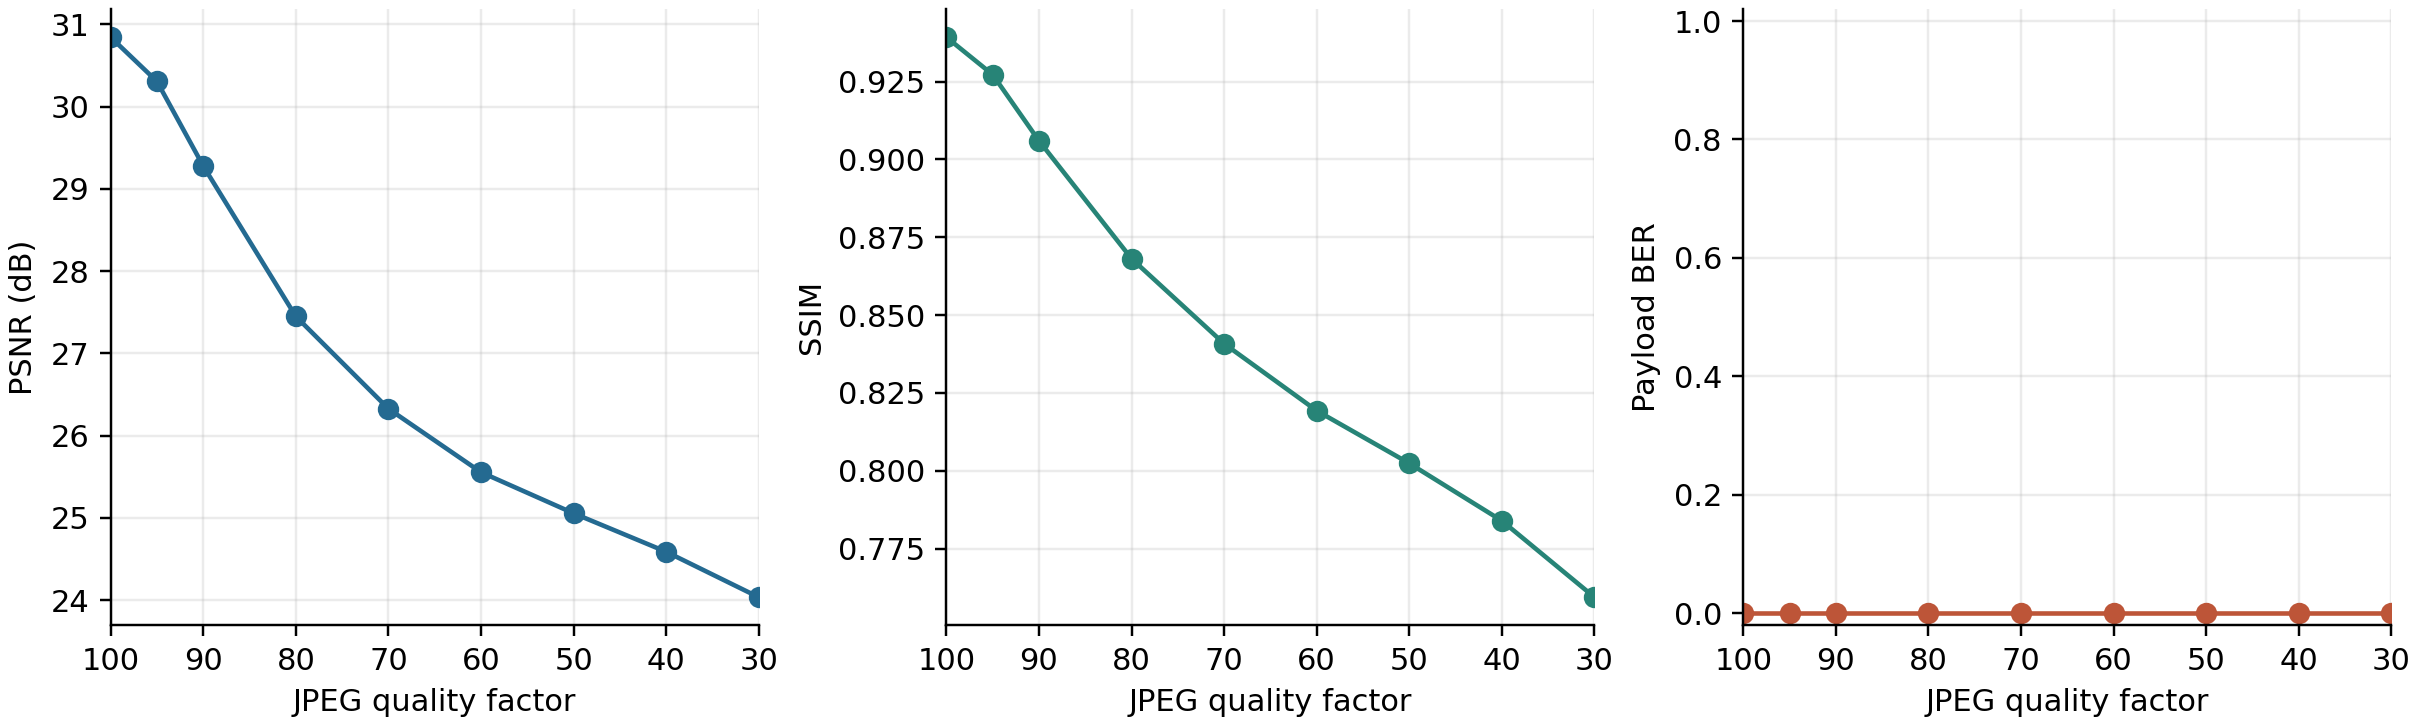
\includegraphics[width=.9\textwidth]{jpeg_sweep.png}
\caption{JPEG quality factors 100, 95, 90, 80, 70, 60, 50, 40, and 30. Lower factors increase distortion. All nine samples in this experiment have BER 0 and valid authentication. Separate axes retain the units of each metric.}
\label{fig:jpeg}
\end{figure}
JPEG Q=100 is still an encode/decode operation, so its PSNR is below that of the
uncompressed marked image. At Q=30, PSNR is 24.03 dB and SSIM is 0.7594, yet payload
recovery succeeds: visual degradation and watermark decoding are related but
different properties. The sweep tests one compression generation on one image, not
repeated transcoding.

\subsection{DSP trade-off: varying quantization strength}
The same image, payload, key, chip length, and coding configuration were held fixed
while $\Delta$ was changed. Each marked image was tested clean, after JPEG Q=50,
and after AWGN with $\sigma=10$ and seed 7.
\begin{table}[H]\centering\footnotesize
\begin{tabular}{rrrrr}
\toprule
$\Delta$ & Clean PSNR (dB) & Clean SSIM & JPEG BER & AWGN BER \\
\midrule
4 & 51.21 & 0.9988 & 0.4722 & 0.5139 \\
6 & 50.02 & 0.9985 & 0.0000 & 1.0000 \\
8 & 48.77 & 0.9981 & 0.0000 & 0.0000 \\
10 & 47.84 & 0.9977 & 0.0000 & 0.0000 \\
12 & 46.97 & 0.9973 & 0.0000 & 0.0000 \\
16 & 45.03 & 0.9959 & 0.0000 & 0.0000 \\
20 & 43.65 & 0.9945 & 0.0000 & 0.0000 \\
\bottomrule
\end{tabular}

\caption{Strength sweep on the single image fixture. All clean cases pass; JPEG passes for $\Delta\ge6$ and AWGN for $\Delta\ge8$ at the sampled settings. Full validity flags are preserved in the JSON data.}
\label{tab:strength}
\end{table}
\begin{figure}[H]
\centering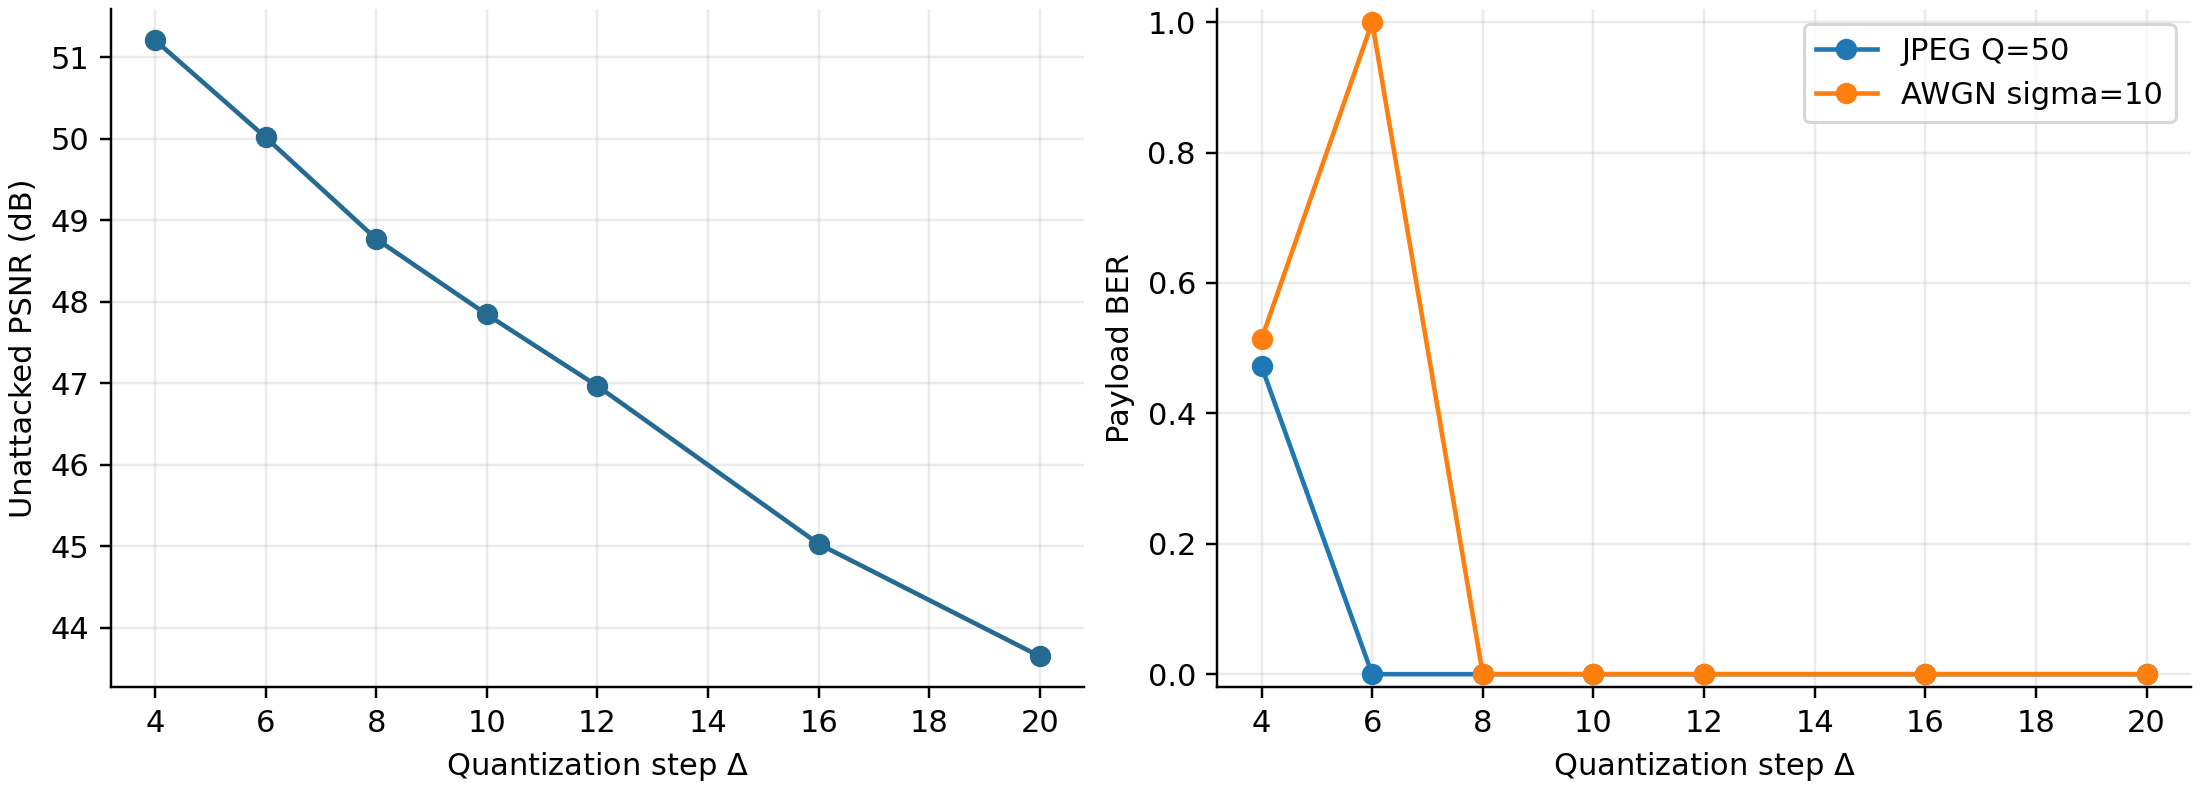
\includegraphics[width=.88\textwidth]{strength_sweep.png}
\caption{Increasing quantization spacing reduces un-attacked PSNR while improving recovery for these selected attacks. A single deterministic sweep cannot establish a universal optimum.}
\end{figure}
At $\Delta=4$, clean PSNR is 51.21 dB but both attacked payloads fail. At $\Delta=12$,
PSNR falls to 46.97 dB and both attacked payloads pass. At $\Delta=20$, PSNR falls
further to 43.65 dB without improving the already-zero BER for these two attacks.
The isolated AWGN failure at $\Delta=6$ is reported as BER 1.0000 by the
length-aware metric; such outcomes reflect nonlinear framing and decoding behavior,
so robustness need not vary smoothly with a parameter.

\section{Measured video results and validation}
\begin{table}[H]\centering\footnotesize
\begin{tabular}{lrrr}
\toprule
Video condition & BER & Valid & Samples \\
\midrule
No additional attack & 0.0000 & Yes & 12 \\
H.264 CRF 28 & 0.0000 & Yes & 12 \\
H.265 CRF 30 & 0.0000 & Yes & 12 \\
Drop every 8th frame & 0.0000 & Yes & 12 \\
Frame-rate conversion 9.00 fps & 0.0000 & Yes & 12 \\
\bottomrule
\end{tabular}

\caption{Recovery from the 24-frame synthetic clip. Samples count low-pass score vectors. Every selected result used phase 0.}
\label{tab:video}
\end{table}
The baseline is already an H.264 encode, so ``no additional attack'' is not a
lossless-channel test. All five conditions recover the 5-byte payload and pass
validation, supporting the feasibility of repeated temporal embedding and combining
for this short fixture. Since every selected phase is zero, the benefit of nonzero
phase search is not demonstrated.

Temporal attacks run through FFmpeg and can include timestamp handling, resampling,
and re-encoding; their labels describe the implemented benchmark operations, not a
validated model of packet loss. Correlated observations from a two-second clip
cannot substitute for trials on diverse scenes.

The full test suite was also run with \code{ffmpeg-python==0.2.0}: \textbf{30 tests
passed}, covering transforms, payload coding, metrics, attacks, image recovery, CLI
manifests, and video integration. Passing tests establish the tested behavior, not
universal robustness.

\section{Limitations and future work}
\begin{enumerate}
\item \textbf{Dataset scope.} Evaluate more photographs and outputs from multiple generators,
with varied texture, motion, resolution, and payload length, and report
distributions and repeated-trial uncertainty.
\item \textbf{Geometric dependence.} Rotation/scale experiments use the original cover.
Synchronization templates or tiled embedding could address cropping and remove the
reference dependence.
\item \textbf{Fixed strength.} A perceptual masking model could adapt $\Delta$ to local
texture, but must be tested against the fixed-strength baseline.
\item \textbf{Temporal scope.} Longer clips, scene cuts, motion, irregular frame removal,
and multiple codec generations are needed, along with video fidelity, flicker,
runtime, and memory measurements.
\item \textbf{Attribution scope.} A public verifier, key management, and trusted identifier
registry are not implemented. A valid payload does not prove the content is
unaltered or that the claimed generator produced it.
\item \textbf{Backend comparison.} STDM and SVD-QIM should be compared at matched payload
rate and distortion.
\end{enumerate}

\section{Conclusion}
The project shows how course concepts combine into a working signal processing
system: Haar analysis gives a multiresolution representation, DCT provides
block-frequency coefficients, keyed projections spread information, and
quantization creates recoverable binary decisions. Soft error-correcting decoding
and temporal combining improve recovery under selected disturbances.

The AI-generated nature image gives 46.97 dB PSNR and 0.9973 SSIM with exact clean
recovery; the rocket photograph gives 47.47 dB and 0.9904 SSIM. Common compression,
noise, and Gaussian-blur cases pass on both. Median filtering and registered rotation
pass only on the rocket photograph; cropping fails on both. The strength
sweep directly illustrates the robustness--distortion trade-off. These findings
support a DSP-based watermarking proof of concept for a future AI-media publishing
workflow, with broader evaluation and provenance infrastructure still required.

\appendix
\section{Reproducing the report}
\subsection{Environment and recorded data}
The run used Windows 11, Python 3.12.7, NumPy 2.2.6, SciPy 1.18.0,
PyWavelets 1.9.0, OpenCV 4.10.0.84, Matplotlib 3.9.2, and
FFmpeg 9.0.2. Environment metadata and the source revision are stored in
\code{data/environment.json}; platform and codec differences can change numeric
results. The video measurements were reused from the previous run (which used
\code{ffmpeg-python 0.2.0}); this image-only rerun did not need that package. No
watermark algorithm was changed for the measurements.

From a clean environment at the repository root:
\begin{lstlisting}
python -m venv .venv
# Activate .venv for your shell, then:
python -m pip install -e ".[dev]"
# Install FFmpeg separately and place ffmpeg/ffprobe on PATH.
python -m pytest -q
python -m report.generate_results
\end{lstlisting}
The last command generates the image/video data, runs the strength sweep, and
writes the figures and LaTeX table fragments. It uses public demonstration keys; in
real use, set a private key and keep it out of logs.

\subsection{LaTeX compilation}
Run \code{pdflatex main.tex} twice (or \code{tectonic main.tex}) from the
\code{report} directory, or upload the source ZIP to Overleaf with \code{main.tex}
as the main file. Figures and table fragments are included; Python is not needed.

\subsection{Artifacts and traceability}
\begin{itemize}
\item \code{main.tex}: editable report, title-page details, derivations, and discussion.
\item \code{image_results.tex} and \code{rocket_results.tex}: numeric image tables.
\item \code{video_results.tex} and \code{strength_results.tex}: numeric video and
strength-sweep tables.
\item \code{figures/}: the generated nature image, rocket photograph, and eight report figures.
\item \code{data/}: JSON for both image attacks, JPEG sweep, video attacks, strength sweep,
summary, and environment.
\item \code{generate_results.py}: reproducible report experiment/plotting script.
\end{itemize}
The DSP overview, soft-score equations, and implementation mapping were checked
against the repository source, and all numbers are fresh measurements.

\begin{thebibliography}{9}
\addcontentsline{toc}{section}{References}
\bibitem{repo} Project source repository, \emph{DSP Course Project: Image and Video
Watermarking}, revision \code{0b74cf3}.\newline
\url{https://github.com/namanshetty25/DSP-Course-Project-Image-Video-Watermarking}
\bibitem{chen} B. Chen and G. W. Wornell, ``Quantization index modulation: A class of
provably good methods for digital watermarking and information embedding,''
\emph{IEEE Transactions on Information Theory}, vol. 47, no. 4, pp. 1423--1443, 2001.\newline
\url{https://sia.mit.edu/wp-content/uploads/2015/04/2001-chen-wornell-it.pdf}
\bibitem{pywt} PyWavelets documentation, ``2D Forward and Inverse Discrete Wavelet
Transform.''\newline
\url{https://pywavelets.readthedocs.io/en/latest/ref/2d-dwt-and-idwt.html}
\bibitem{scipy} SciPy documentation, ``Discrete Fourier Transforms
(scipy.fft),'' discrete cosine transform section.\newline
\url{https://docs.scipy.org/doc/scipy/tutorial/fft.html}
\bibitem{rocket} scikit-image documentation, ``rocket: SpaceX launch photograph, public domain.''\newline
\href{https://scikit-image.org/docs/stable/api/skimage.data.html#skimage.data.rocket}{scikit-image rocket dataset documentation}
\end{thebibliography}
\end{document}
